\documentclass[•]{article}
\usepackage{pgfplots}

\author{John Niemeyer\\JJNB78@mst.edu}
\title{COMP SCI 5401 FS2017 Assignment 2a}

\begin{document}
\maketitle

\section{Evaluations vs. Fitness graph}
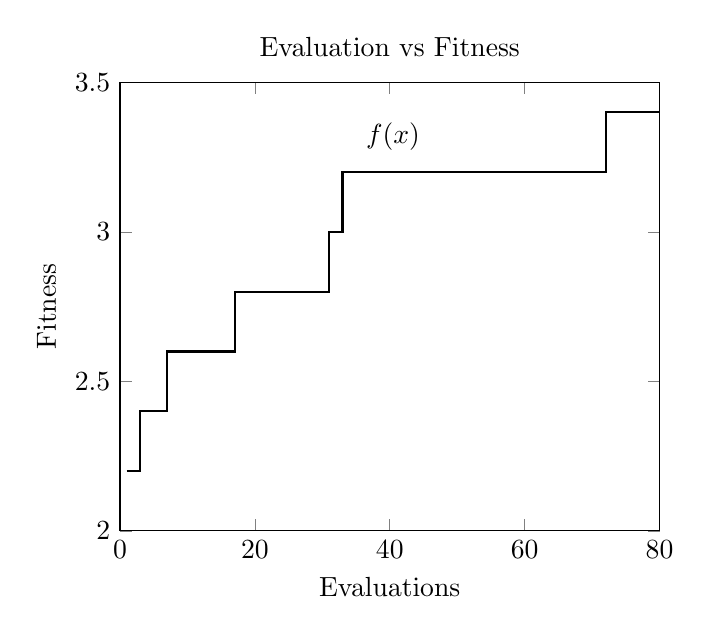
\begin{tikzpicture}
\begin{axis}[
	title = {Evaluation vs Fitness},
    xlabel={Evaluations},
    ylabel={Fitness},
    xmin=0, xmax=80,
    ymin=2,ymax=3.5,
    xtick={0, 20, 40, 60, 80},
    ytick={2, 2.5, 3, 3.5},
    ]
\addplot[const plot, no marks, thick] coordinates {(1, 2.2) (3, 2.4) (7, 2.6) (17, 2.8) (31, 3.0) (33, 3.2) (72, 3.4) (80, 3.4)} node[above,pos=.50,black] {$f(x)$};
\end{axis}
\end{tikzpicture}
\end{document}